\documentclass{standalone}
\usepackage{tikz}
\usetikzlibrary{patterns, positioning}
\usepackage[sfdefault]{ClearSans} %% option 'sfdefault' activates Clear Sans as the default text font
\usepackage[T1]{fontenc}

\begin{document}
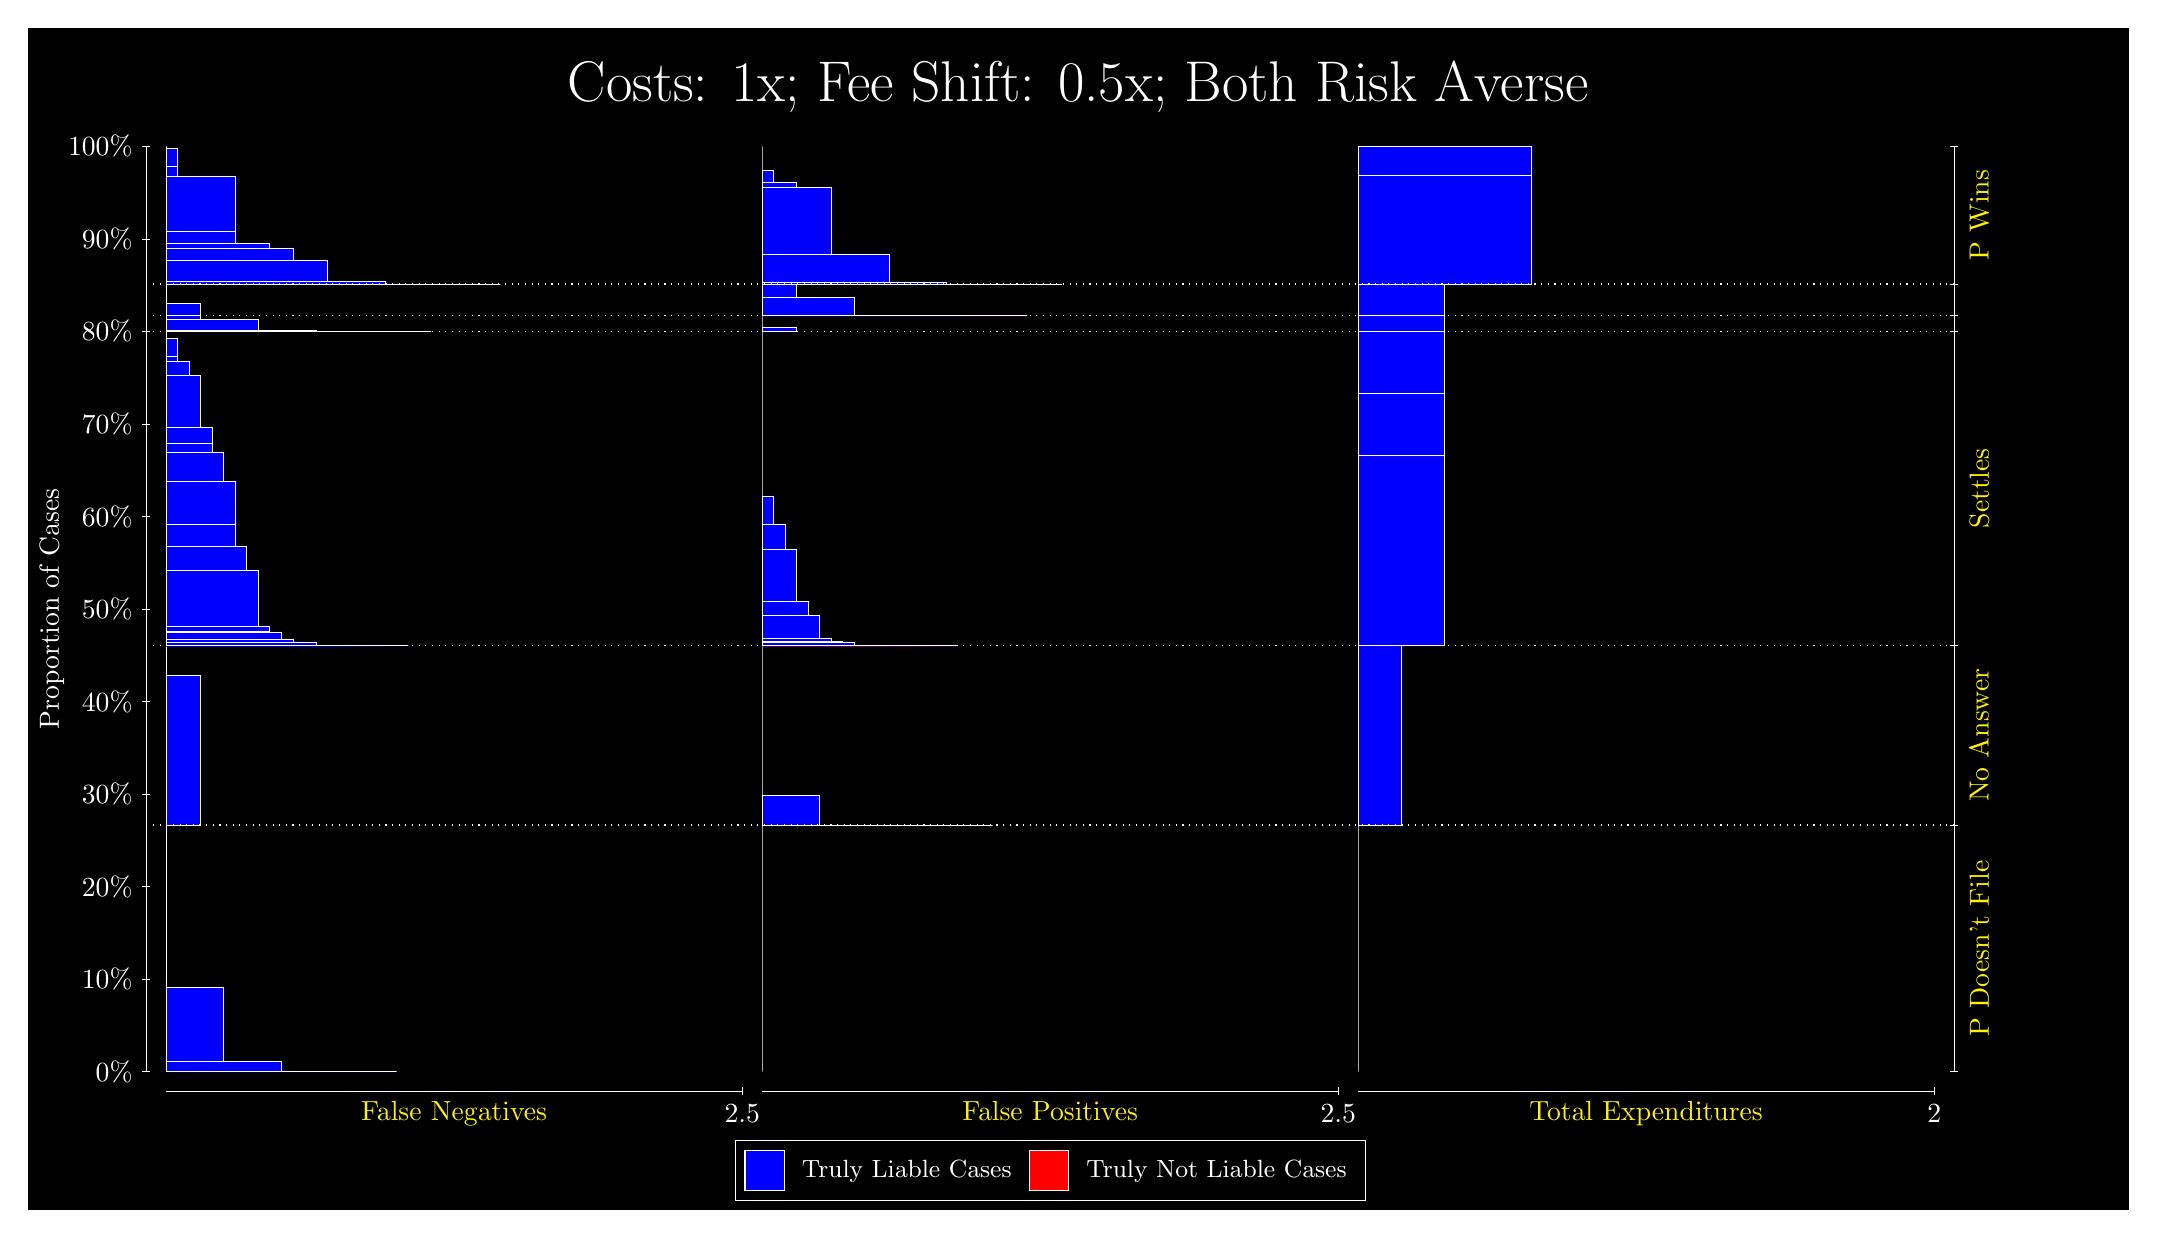
\begin{tikzpicture}
\draw[fill=black] (0,0) rectangle (26.667,15);
\draw[text=white] (0,13.5) rectangle (26.667,15) node[midway] {\huge Costs: 1x; Fee Shift: 0.5x; Both Risk Averse};
\draw[white, very thin] (1.5,1.75) -- (1.5,13.5);
\node[rotate=90, text=white, anchor=center] at (0.3, 7.625) {Proportion of Cases};
\draw[white, very thin] (1.45,1.75) -- (1.55,1.75);
\node[text=white, anchor=east] at (1.45, 1.75) {0\%};
\draw[white, very thin] (1.45,2.925) -- (1.55,2.925);
\node[text=white, anchor=east] at (1.45, 2.925) {10\%};
\draw[white, very thin] (1.45,4.1) -- (1.55,4.1);
\node[text=white, anchor=east] at (1.45, 4.1) {20\%};
\draw[white, very thin] (1.45,5.275) -- (1.55,5.275);
\node[text=white, anchor=east] at (1.45, 5.275) {30\%};
\draw[white, very thin] (1.45,6.45) -- (1.55,6.45);
\node[text=white, anchor=east] at (1.45, 6.45) {40\%};
\draw[white, very thin] (1.45,7.625) -- (1.55,7.625);
\node[text=white, anchor=east] at (1.45, 7.625) {50\%};
\draw[white, very thin] (1.45,8.8) -- (1.55,8.8);
\node[text=white, anchor=east] at (1.45, 8.8) {60\%};
\draw[white, very thin] (1.45,9.975) -- (1.55,9.975);
\node[text=white, anchor=east] at (1.45, 9.975) {70\%};
\draw[white, very thin] (1.45,11.15) -- (1.55,11.15);
\node[text=white, anchor=east] at (1.45, 11.15) {80\%};
\draw[white, very thin] (1.45,12.325) -- (1.55,12.325);
\node[text=white, anchor=east] at (1.45, 12.325) {90\%};
\draw[white, very thin] (1.45,13.5) -- (1.55,13.5);
\node[text=white, anchor=east] at (1.45, 13.5) {100\%};

\draw[white, very thin] (24.457,1.75) -- (24.457,13.5);
\draw[white, very thin] (24.407,1.75) -- (24.507,1.75);
\node[anchor=west] at (24.407, 1.75) {};
\draw[white, very thin] (24.407,4.8805) -- (24.507,4.8805);
\node[anchor=west] at (24.407, 4.8805) {};
\draw[white, very thin] (24.407,7.1603) -- (24.507,7.1603);
\node[anchor=west] at (24.407, 7.1603) {};
\draw[white, very thin] (24.407,11.153) -- (24.507,11.153);
\node[anchor=west] at (24.407, 11.153) {};
\draw[white, very thin] (24.407,11.348) -- (24.507,11.348);
\node[anchor=west] at (24.407, 11.348) {};
\draw[white, very thin] (24.407,11.752) -- (24.507,11.752);
\node[anchor=west] at (24.407, 11.752) {};
\draw[white, very thin] (24.407,13.5) -- (24.507,13.5);
\node[anchor=west] at (24.407, 13.5) {};

\draw[white, very thin, fill=blue] (1.75,1.75) rectangle (4.6775,1.75);
\draw[white, very thin, fill=blue] (1.75,1.75) rectangle (3.9457,1.7511);
\draw[white, very thin, fill=blue] (1.75,1.7511) rectangle (3.2138,1.8843);
\draw[white, very thin, fill=blue] (1.75,1.8843) rectangle (2.4819,2.8192);
\draw[white, very thin, fill=red] (1.75,2.8192) rectangle (1.75,2.8192);
\draw[white, very thin, fill=blue] (1.75,2.8192) rectangle (1.75,4.8805);
\draw[white, very thin, fill=blue] (1.75,4.8805) rectangle (2.1891,6.7873);
\draw[white, very thin, fill=red] (1.75,6.7873) rectangle (1.75,6.7873);
\draw[white, very thin, fill=blue] (1.75,6.7873) rectangle (1.75,7.1603);
\draw[white, very thin, fill=blue] (1.75,7.1603) rectangle (4.8239,7.1603);
\draw[white, very thin, fill=blue] (1.75,7.1603) rectangle (4.5312,7.1603);
\draw[white, very thin, fill=blue] (1.75,7.1603) rectangle (4.2384,7.1603);
\draw[white, very thin, fill=blue] (1.75,7.1603) rectangle (4.092,7.1603);
\draw[white, very thin, fill=blue] (1.75,7.1603) rectangle (3.9457,7.1605);
\draw[white, very thin, fill=blue] (1.75,7.1605) rectangle (3.7993,7.1606);
\draw[white, very thin, fill=blue] (1.75,7.1606) rectangle (3.6529,7.1956);
\draw[white, very thin, fill=blue] (1.75,7.1956) rectangle (3.5065,7.206);
\draw[white, very thin, fill=blue] (1.75,7.206) rectangle (3.3602,7.2455);
\draw[white, very thin, fill=blue] (1.75,7.2455) rectangle (3.2138,7.3274);
\draw[white, very thin, fill=blue] (1.75,7.3274) rectangle (3.0674,7.3366);
\draw[white, very thin, fill=blue] (1.75,7.3366) rectangle (3.0674,7.3988);
\draw[white, very thin, fill=blue] (1.75,7.3988) rectangle (2.921,8.1103);
\draw[white, very thin, fill=blue] (1.75,8.1103) rectangle (2.7746,8.4217);
\draw[white, very thin, fill=blue] (1.75,8.4217) rectangle (2.6283,8.7023);
\draw[white, very thin, fill=blue] (1.75,8.7023) rectangle (2.6283,9.2523);
\draw[white, very thin, fill=blue] (1.75,9.2523) rectangle (2.4819,9.6115);
\draw[white, very thin, fill=blue] (1.75,9.6115) rectangle (2.3355,9.7344);
\draw[white, very thin, fill=blue] (1.75,9.7344) rectangle (2.3355,9.9313);
\draw[white, very thin, fill=blue] (1.75,9.9313) rectangle (2.1891,10.596);
\draw[white, very thin, fill=blue] (1.75,10.596) rectangle (2.0428,10.774);
\draw[white, very thin, fill=blue] (1.75,10.774) rectangle (1.8964,10.837);
\draw[white, very thin, fill=blue] (1.75,10.837) rectangle (1.8964,11.061);
\draw[white, very thin, fill=blue] (1.75,11.061) rectangle (1.75,11.061);
\draw[white, very thin, fill=red] (1.75,11.061) rectangle (1.75,11.061);
\draw[white, very thin, fill=blue] (1.75,11.061) rectangle (1.75,11.153);
\draw[white, very thin, fill=blue] (1.75,11.153) rectangle (5.1167,11.153);
\draw[white, very thin, fill=blue] (1.75,11.153) rectangle (4.3848,11.153);
\draw[white, very thin, fill=blue] (1.75,11.153) rectangle (3.6529,11.169);
\draw[white, very thin, fill=blue] (1.75,11.169) rectangle (2.921,11.302);
\draw[white, very thin, fill=blue] (1.75,11.302) rectangle (2.1891,11.348);
\draw[white, very thin, fill=red] (1.75,11.348) rectangle (1.75,11.348);
\draw[white, very thin, fill=blue] (1.75,11.348) rectangle (2.1891,11.511);
\draw[white, very thin, fill=red] (1.75,11.511) rectangle (1.75,11.511);
\draw[white, very thin, fill=blue] (1.75,11.511) rectangle (1.75,11.752);
\draw[white, very thin, fill=blue] (1.75,11.752) rectangle (5.9949,11.752);
\draw[white, very thin, fill=blue] (1.75,11.752) rectangle (5.2631,11.752);
\draw[white, very thin, fill=blue] (1.75,11.752) rectangle (4.8239,11.752);
\draw[white, very thin, fill=blue] (1.75,11.752) rectangle (4.5312,11.787);
\draw[white, very thin, fill=blue] (1.75,11.787) rectangle (4.092,11.787);
\draw[white, very thin, fill=blue] (1.75,11.787) rectangle (3.7993,12.058);
\draw[white, very thin, fill=blue] (1.75,12.058) rectangle (3.3602,12.209);
\draw[white, very thin, fill=blue] (1.75,12.209) rectangle (3.0674,12.271);
\draw[white, very thin, fill=blue] (1.75,12.271) rectangle (2.6283,12.415);
\draw[white, very thin, fill=blue] (1.75,12.415) rectangle (2.6283,13.121);
\draw[white, very thin, fill=blue] (1.75,13.121) rectangle (2.3355,13.121);
\draw[white, very thin, fill=blue] (1.75,13.121) rectangle (1.8964,13.248);
\draw[white, very thin, fill=blue] (1.75,13.248) rectangle (1.8964,13.478);
\draw[white, very thin, fill=red] (1.75,13.478) rectangle (1.75,13.478);
\draw[white, very thin, fill=blue] (1.75,13.478) rectangle (1.75,13.5);
\draw[white, very thin, fill=red] (9.3189,1.75) rectangle (9.3189,1.75);
\draw[white, very thin, fill=blue] (9.3189,1.75) rectangle (9.3189,4.8805);
\draw[white, very thin, fill=red] (9.3189,4.8805) rectangle (12.246,4.8805);
\draw[white, very thin, fill=blue] (9.3189,4.8805) rectangle (12.246,4.8805);
\draw[white, very thin, fill=blue] (9.3189,4.8805) rectangle (11.515,4.8805);
\draw[white, very thin, fill=blue] (9.3189,4.8805) rectangle (10.783,4.8835);
\draw[white, very thin, fill=blue] (9.3189,4.8835) rectangle (10.051,5.2535);
\draw[white, very thin, fill=blue] (9.3189,5.2535) rectangle (9.3189,7.1603);
\draw[white, very thin, fill=red] (9.3189,7.1603) rectangle (11.807,7.1603);
\draw[white, very thin, fill=blue] (9.3189,7.1603) rectangle (11.807,7.1603);
\draw[white, very thin, fill=red] (9.3189,7.1603) rectangle (11.515,7.1603);
\draw[white, very thin, fill=blue] (9.3189,7.1603) rectangle (11.515,7.1603);
\draw[white, very thin, fill=red] (9.3189,7.1603) rectangle (11.222,7.1603);
\draw[white, very thin, fill=blue] (9.3189,7.1603) rectangle (11.222,7.1604);
\draw[white, very thin, fill=blue] (9.3189,7.1604) rectangle (11.075,7.1604);
\draw[white, very thin, fill=red] (9.3189,7.1604) rectangle (10.929,7.1604);
\draw[white, very thin, fill=blue] (9.3189,7.1604) rectangle (10.929,7.1608);
\draw[white, very thin, fill=red] (9.3189,7.1608) rectangle (10.929,7.1608);
\draw[white, very thin, fill=blue] (9.3189,7.1608) rectangle (10.929,7.1608);
\draw[white, very thin, fill=blue] (9.3189,7.1608) rectangle (10.783,7.1609);
\draw[white, very thin, fill=red] (9.3189,7.1609) rectangle (10.636,7.1609);
\draw[white, very thin, fill=blue] (9.3189,7.1609) rectangle (10.636,7.1654);
\draw[white, very thin, fill=blue] (9.3189,7.1654) rectangle (10.49,7.2002);
\draw[white, very thin, fill=red] (9.3189,7.2002) rectangle (10.344,7.2002);
\draw[white, very thin, fill=blue] (9.3189,7.2002) rectangle (10.344,7.2178);
\draw[white, very thin, fill=blue] (9.3189,7.2178) rectangle (10.197,7.2524);
\draw[white, very thin, fill=blue] (9.3189,7.2524) rectangle (10.197,7.2528);
\draw[white, very thin, fill=red] (9.3189,7.2528) rectangle (10.051,7.2528);
\draw[white, very thin, fill=blue] (9.3189,7.2528) rectangle (10.051,7.5396);
\draw[white, very thin, fill=blue] (9.3189,7.5396) rectangle (9.9044,7.7176);
\draw[white, very thin, fill=blue] (9.3189,7.7176) rectangle (9.758,8.3823);
\draw[white, very thin, fill=blue] (9.3189,8.3823) rectangle (9.6116,8.7022);
\draw[white, very thin, fill=blue] (9.3189,8.7022) rectangle (9.4652,9.0509);
\draw[white, very thin, fill=blue] (9.3189,9.0509) rectangle (9.4652,9.0614);
\draw[white, very thin, fill=blue] (9.3189,9.0614) rectangle (9.3189,11.153);
\draw[white, very thin, fill=red] (9.3189,11.153) rectangle (9.758,11.153);
\draw[white, very thin, fill=blue] (9.3189,11.153) rectangle (9.758,11.199);
\draw[white, very thin, fill=blue] (9.3189,11.199) rectangle (9.3189,11.348);
\draw[white, very thin, fill=red] (9.3189,11.348) rectangle (12.686,11.348);
\draw[white, very thin, fill=blue] (9.3189,11.348) rectangle (12.686,11.348);
\draw[white, very thin, fill=blue] (9.3189,11.348) rectangle (11.954,11.348);
\draw[white, very thin, fill=blue] (9.3189,11.348) rectangle (11.222,11.355);
\draw[white, very thin, fill=blue] (9.3189,11.355) rectangle (10.49,11.588);
\draw[white, very thin, fill=blue] (9.3189,11.588) rectangle (9.758,11.752);
\draw[white, very thin, fill=red] (9.3189,11.752) rectangle (13.125,11.752);
\draw[white, very thin, fill=blue] (9.3189,11.752) rectangle (13.125,11.752);
\draw[white, very thin, fill=red] (9.3189,11.752) rectangle (12.393,11.752);
\draw[white, very thin, fill=blue] (9.3189,11.752) rectangle (12.393,11.752);
\draw[white, very thin, fill=red] (9.3189,11.752) rectangle (11.661,11.752);
\draw[white, very thin, fill=blue] (9.3189,11.752) rectangle (11.661,11.774);
\draw[white, very thin, fill=red] (9.3189,11.774) rectangle (11.222,11.774);
\draw[white, very thin, fill=blue] (9.3189,11.774) rectangle (11.222,11.774);
\draw[white, very thin, fill=red] (9.3189,11.774) rectangle (10.929,11.774);
\draw[white, very thin, fill=blue] (9.3189,11.774) rectangle (10.929,12.131);
\draw[white, very thin, fill=red] (9.3189,12.131) rectangle (10.49,12.131);
\draw[white, very thin, fill=blue] (9.3189,12.131) rectangle (10.49,12.131);
\draw[white, very thin, fill=blue] (9.3189,12.131) rectangle (10.197,12.981);
\draw[white, very thin, fill=blue] (9.3189,12.981) rectangle (9.758,13.041);
\draw[white, very thin, fill=red] (9.3189,13.041) rectangle (9.758,13.041);
\draw[white, very thin, fill=blue] (9.3189,13.041) rectangle (9.758,13.043);
\draw[white, very thin, fill=blue] (9.3189,13.043) rectangle (9.4652,13.193);
\draw[white, very thin, fill=blue] (9.3189,13.193) rectangle (9.3189,13.5);
\draw[white, very thin, fill=red] (16.888,1.75) rectangle (16.888,1.75);
\draw[white, very thin, fill=blue] (16.888,1.75) rectangle (16.888,4.8805);
\draw[white, very thin, fill=red] (16.888,4.8805) rectangle (17.437,4.8805);
\draw[white, very thin, fill=blue] (16.888,4.8805) rectangle (17.437,7.1603);
\draw[white, very thin, fill=red] (16.888,7.1603) rectangle (17.986,7.1603);
\draw[white, very thin, fill=blue] (16.888,7.1603) rectangle (17.986,9.5719);
\draw[white, very thin, fill=red] (16.888,9.5719) rectangle (17.986,9.5719);
\draw[white, very thin, fill=blue] (16.888,9.5719) rectangle (17.986,10.368);
\draw[white, very thin, fill=red] (16.888,10.368) rectangle (17.986,10.368);
\draw[white, very thin, fill=blue] (16.888,10.368) rectangle (17.986,11.153);
\draw[white, very thin, fill=red] (16.888,11.153) rectangle (17.986,11.153);
\draw[white, very thin, fill=blue] (16.888,11.153) rectangle (17.986,11.348);
\draw[white, very thin, fill=red] (16.888,11.348) rectangle (17.986,11.348);
\draw[white, very thin, fill=blue] (16.888,11.348) rectangle (17.986,11.752);
\draw[white, very thin, fill=red] (16.888,11.752) rectangle (19.083,11.752);
\draw[white, very thin, fill=blue] (16.888,11.752) rectangle (19.083,13.131);
\draw[white, very thin, fill=red] (16.888,13.131) rectangle (19.083,13.131);
\draw[white, very thin, fill=blue] (16.888,13.131) rectangle (19.083,13.5);
\draw[white, dotted] (1.5,4.8805) -- (24.457,4.8805);
\draw[white, dotted] (1.5,7.1603) -- (24.457,7.1603);
\draw[white, dotted] (1.5,11.153) -- (24.457,11.153);
\draw[white, dotted] (1.5,11.348) -- (24.457,11.348);
\draw[white, dotted] (1.5,11.752) -- (24.457,11.752);
\draw[white, very thin] (1.75,1.5) -- (9.0689,1.5);
\node[text=yellow, anchor=north] at (5.4094, 1.5) {False Negatives};
\draw[white, very thin] (9.0689,1.45) -- (9.0689,1.55);
\node[text=white, anchor=north] at (9.0689, 1.45) {2.5};

\draw[white, very thin] (9.3189,1.5) -- (16.638,1.5);
\node[text=yellow, anchor=north] at (12.978, 1.5) {False Positives};
\draw[white, very thin] (16.638,1.45) -- (16.638,1.55);
\node[text=white, anchor=north] at (16.638, 1.45) {2.5};

\draw[white, very thin] (16.888,1.5) -- (24.207,1.5);
\node[text=yellow, anchor=north] at (20.547, 1.5) {Total Expenditures};
\draw[white, very thin] (24.207,1.45) -- (24.207,1.55);
\node[text=white, anchor=north] at (24.207, 1.45) {2};

\node[text=yellow, centered, rotate=90] at (24.777, 3.3152) {P Doesn't File};
\node[text=yellow, centered, rotate=90] at (24.777, 6.0204) {No Answer};
\node[text=yellow, centered, rotate=90] at (24.777, 9.1568) {Settles};


\node[text=yellow, centered, rotate=90] at (24.777, 12.626) {P Wins};

\draw (12.978300999999998,1.5) node[draw=none] (baseCoordinate) {};
\begin{scope}[align=center]
        \matrix[scale=0.5, draw=white, below=0.5cm of baseCoordinate, nodes={draw}, column sep=0.1cm]{
            \node[rectangle, draw, minimum width=0.5cm, minimum height=0.5cm, fill=blue] {}; &
            \node[draw=none, font=\small, text=white] (B) {Truly Liable Cases}; &
            \node[rectangle, draw, minimum width=0.5cm, minimum height=0.5cm, fill=red] {}; &
            \node[draw=none, font=\small, text=white] (B) {Truly Not Liable Cases}; \\
            };
\end{scope}

\end{tikzpicture}
\end{document}